% !TEX root = main.tex
\documentclass[aspectratio=169,11pt,xcolor={dvipsnames},hyperref={pdftex,pdfpagemode=UseNone,hidelinks,pdfdisplaydoctitle=true},usepdftitle=false]{beamer}
\usepackage{../include/slide}
\usepackage{tikz}

\title{Multi-Robot Waypoint Inspection Planning with Mixed Integer Linear Programming Project}
\author{Juan Carlos Cruz - ira406}
\date{ME 6033 Linear and Mixed Integer Optimization}
\begin{document}
    
    \begin{frame}
      \titlepage
      May 20.48
    \end{frame}
    
    \begin{frame}{Introduction}
      \begin{columns}[c]
        \begin{column}{0.48\textwidth}
          \begin{itemize}
            \item Based on previous work done in an outdoor concrete inspection multirobot framework
            \item Precast concrete elements require efficient inspection methods after being transported to a site
            \item Multi-robot approach:
              \begin{itemize}
                \item Aerial robots locate targets
                \item Ground robots perform detailed inspections
              \end{itemize}
            \item For this project wanted to see if we could extend this idea to planning of multiple robots across an inspection site
          \end{itemize}
          
        \end{column}

        \begin{column}{0.48\textwidth}

          \begin{figure}
            \centering
            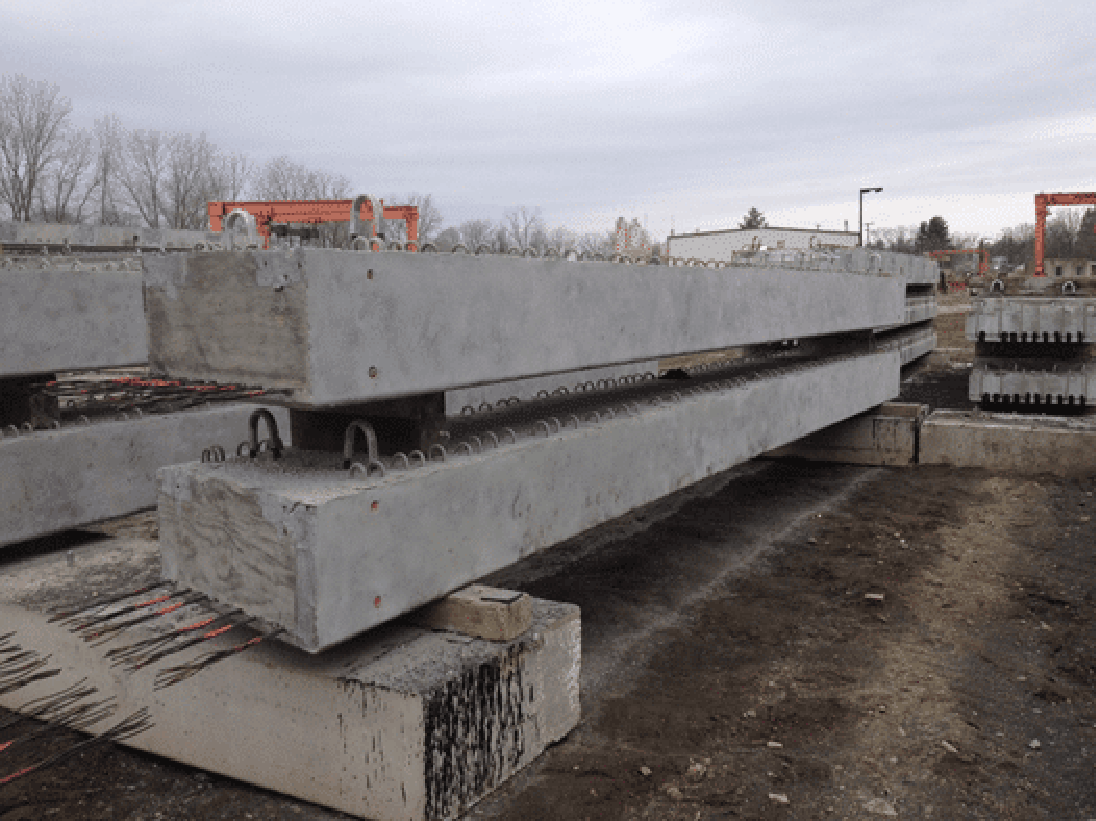
\includegraphics[scale=0.35]{figures/concrete.pdf}
          \end{figure}
              
        \end{column}
      \end{columns}

    \end{frame}

    \begin{frame}{Problem Description}
      \begin{itemize}
        \item Two robot types with variable quantity: aerial and ground mobile robots
        \item Inspection targets as waypoints in a 2D plane $(x,y)$
        \item Depot location for each robot type. Must leave and return to this location.
        \item Sequential operation:
          \begin{itemize}
            \item Aerial robots verify waypoint location first
            \item Ground robots perform detailed inspection second
          \end{itemize}
        \item Robot parameters (defined by robot type):
          \begin{itemize}
            \item Fixed speeds (meters/minute)
            \item Limited operation time (battery life time after leaving depot)
            \item Required inspection time at waypoints
          \end{itemize}
      \end{itemize}
    \end{frame}

    \begin{frame}{Literature Review}
      \begin{itemize}
        \item Prior works demonstrate multi-robot planning applications
        \item Problem resembles multiple traveling salesman problem (mTSP)
        \item Traditional MILP for mTSP:
          \begin{itemize}
            \item Routing variables 
            \item Subtour elimination constraints
          \end{itemize}
        \item Initially tried this approach but solving time was too slow and larger problems became infeasible (likely implementation error) so used a simplification
        \item Route approximation: roundtrip distances from depot to waypoints estimate travel times
      \end{itemize}
    \end{frame}

  \begin{frame}{Mathematical Model - Overview}
    \begin{itemize}
      \item Mixed Integer Linear Programming (MILP) formulation
      \item Objective: Maximize number of waypoints inspected
      \item Constraints consider:
        \begin{itemize}
          \item Robot assignment to waypoints
          \item Sequential operations (aerial robots first, then ground)
          \item Time limitations from battery endurance
          \item Travel speed and inspection time requirements
        \end{itemize}
      \item Approximates routes using roundtrip distances from depot
    \end{itemize}
  \end{frame}

  \begin{frame}{Mathematical Model - Sets and Indices}
    \begin{itemize}
      \item $N$: Set of all waypoints indexed by $i \in \{1, 2, \ldots, n\}$
      \item $K$: Set of aerial robots indexed by $k \in \{1, 2, \ldots, k_{\max}\}$
      \item $L$: Set of ground robots indexed by $l \in \{1, 2, \ldots, l_{\max}\}$
      \item $d_A$: Aerial robot depot
      \item $d_G$: Ground robot depot
    \end{itemize}
  \end{frame}

  \begin{frame}{Mathematical Model - Parameters}
    \begin{columns}[c]
      \begin{column}{0.48\textwidth}
        \begin{itemize}
          \item $p_i$: Location of waypoint $i \in N$
          \item $p_{d_A}$: Location of aerial robot depot
          \item $p_{d_G}$: Location of ground robot depot
          \item $\text{dist}(i,j)$: Euclidean distance between locations $i$ and $j$
          \item $s_A$: Speed of aerial robots (m/min)
        \end{itemize}
      \end{column}
      \begin{column}{0.48\textwidth}
        \begin{itemize}
          \item $s_G$: Speed of ground robots (m/min)
          \item $t_A^{\text{insp}}$: Inspection time for aerial robots (min)
          \item $t_G^{\text{insp}}$: Inspection time for ground robots (min)
          \item $T_A^{\max}$: Maximum operation time for aerial robots (min)
          \item $T_G^{\max}$: Maximum operation time for ground robots (min)
        \end{itemize}
      \end{column}
    \end{columns}
  \end{frame}

  \begin{frame}{Mathematical Model - Derived Parameters}
    \begin{itemize}
      \item $t_{ij}^{A} = \frac{\text{dist}(i,j)}{s_A}$: Travel time for aerial robots from $i$ to $j$ (min)
      \item $t_{ij}^{G} = \frac{\text{dist}(i,j)}{s_G}$: Travel time for ground robots from $i$ to $j$ (min)
      \item $M_A$: Big-M value for aerial robot time constraints\\
            Calculated as $T_A^{\max}$ + max($t_{ij}^{A}$) + $t_A^{\text{insp}}$
      \item $M_G$: Big-M value for ground robot time constraints\\
            Calculated as $T_G^{\max}$ + max($t_{ij}^{G}$) + $t_G^{\text{insp}}$
    \end{itemize}
  \end{frame}

  \begin{frame}{Mathematical Model - Decision Variables}
    \begin{columns}[c]
      \begin{column}{0.48\textwidth}
        \begin{itemize}
          \item $w_i^{a,k}$: Binary variable equals 1 if aerial robot $k$ visits waypoint $i$
          \item $w_i^{g,l}$: Binary variable equals 1 if ground robot $l$ visits waypoint $i$
          \item $a_i^k$: Time when aerial robot $k$ completes inspection at waypoint $i$
        \end{itemize}
      \end{column}
      \begin{column}{0.48\textwidth}
        \begin{itemize}
          \item $g_i^l$: Time when ground robot $l$ completes inspection at waypoint $i$
          \item $\text{use}_k^a$: Binary variable equals 1 if aerial robot $k$ is used
          \item $\text{use}_l^g$: Binary variable equals 1 if ground robot $l$ is used
          \item $z_i^{k,l}$: Binary variable equals 1 if ground robot $l$ visits waypoint $i$ after aerial robot $k$
        \end{itemize}
      \end{column}
    \end{columns}
  \end{frame}

  \begin{frame}{Mathematical Model - Objective Function}
    \begin{itemize}
      \item Goal: Maximize the number of waypoints visited by ground robots
    \end{itemize}
    \begin{align}
      \text{Maximize} \sum_{i \in N}\sum_{l \in L} w_i^{g,l}
    \end{align}
    \begin{itemize}
      \item A waypoint is only considered completely inspected when a ground robot has visited it
      \item Aerial robot visits alone do not contribute to the objective
    \end{itemize}
  \end{frame}

  \begin{frame}{Mathematical Model - Assignment Constraints}
    \begin{itemize}
      \item Each waypoint can be assigned to at most one aerial robot:
      \begin{equation}
        \sum_{k \in K} w_i^{a,k} \leq 1 \quad \forall i \in N
      \end{equation}
      
      \item Each waypoint can be assigned to at most one ground robot:
      \begin{equation}
        \sum_{l \in L} w_i^{g,l} \leq 1 \quad \forall i \in N
      \end{equation}
    \end{itemize}
  \end{frame}

  \begin{frame}{Mathematical Model - Robot Usage Constraints}
    \begin{itemize}
      \item A robot is used if it visits at least one waypoint:
      \begin{align}
        \sum_{i \in N} w_i^{a,k} \geq \text{use}_k^a \quad \forall k \in K\\
        \sum_{i \in N} w_i^{g,l} \geq \text{use}_l^g \quad \forall l \in L
      \end{align}
      
      \item A robot is used only if it visits at least one waypoint:
      \begin{align}
        \sum_{i \in N} w_i^{a,k} \leq n \cdot \text{use}_k^a \quad \forall k \in K\\
        \sum_{i \in N} w_i^{g,l} \leq n \cdot \text{use}_l^g \quad \forall l \in L
      \end{align}
    \end{itemize}
  \end{frame}

  \begin{frame}{Mathematical Model - Precedence Constraints (1)}
    \begin{itemize}
      \item Ground robots can only visit waypoints already visited by aerial robots:
      \begin{equation}
        w_i^{g,l} \leq \sum_{k \in K} w_i^{a,k} \quad \forall i \in N, \forall l \in L
      \end{equation}
      
      \item Ground robot's inspection must occur after aerial robot's inspection:
      \begin{equation}
        g_i^l \geq a_i^k - M_G \cdot (1 - z_i^{k,l}) - M_G \cdot (2 - \text{use}_k^a - \text{use}_l^g) \quad \forall i, k, l
      \end{equation}
    \end{itemize}
  \end{frame}

  \begin{frame}{Mathematical Model - Precedence Constraints (2)}
    Constraints on $z_i^{k,l}$ (linking variable for timing precedence):
    \begin{align}
      z_i^{k,l} &\leq w_i^{g,l} \quad \forall i \in N, \forall k \in K, \forall l \in L\\
      z_i^{k,l} &\leq w_i^{a,k} \quad \forall i \in N, \forall k \in K, \forall l \in L\\
      z_i^{k,l} &\leq \text{use}_k^a \quad \forall i \in N, \forall k \in K, \forall l \in L\\
      z_i^{k,l} &\leq \text{use}_l^g \quad \forall i \in N, \forall k \in K, \forall l \in L
    \end{align}
    \begin{align}
      z_i^{k,l} \geq w_i^{g,l} + w_i^{a,k} + \text{use}_k^a + \text{use}_l^g - 3 \quad \forall i, k, l
    \end{align}
  \end{frame}

  \begin{frame}{Mathematical Model - Time Constraints (1)}
    \begin{itemize}
      \item Minimum inspection time at waypoints:
      \begin{align}
        a_i^k &\geq t_A^{\text{insp}} \cdot w_i^{a,k} \quad \forall i \in N, \forall k \in K\\
        g_i^l &\geq t_G^{\text{insp}} \cdot w_i^{g,l} \quad \forall i \in N, \forall l \in L
      \end{align}
    \end{itemize}
  \end{frame}

  \begin{frame}{Mathematical Model - Time Constraints (2)}
    \begin{itemize}
      \item Maximum operation time constraints:
      \begin{align}
        a_i^k + t_{i,d_A}^{A} \cdot w_i^{a,k} &\leq T_A^{\max} + M_A \cdot (1 - w_i^{a,k}) \\
        &\forall i \in N, \forall k \in K
      \end{align}
      
      \begin{align}
        g_i^l + t_{i,d_G}^{G} \cdot w_i^{g,l} &\leq T_G^{\max} + M_G \cdot (1 - w_i^{g,l}) \\
        &\forall i \in N, \forall l \in L
      \end{align}
    \end{itemize}
  \end{frame}

  \begin{frame}{Mathematical Model - Route Length Constraints}
    \begin{itemize}
      \item Total mission time estimation (route approximation):
      \begin{align}
        \sum_{i \in N} w_i^{a,k} \cdot \left( 2 \cdot t_{d_A,i}^{A}\right) + \sum_{i \in N} w_i^{a,k} \cdot t_A^{\text{insp}} \\ 
        \leq T_A^{\max} + M_A \cdot (1 - \text{use}_k^a) \quad \forall k \in K
      \end{align}
      
      \begin{align}
        \sum_{i \in N} w_i^{g,l} \cdot \left( 2 \cdot t_{d_G,i}^{G}\right) + \sum_{i \in N} w_i^{g,l} \cdot t_G^{\text{insp}} \\
        \leq T_G^{\max} + M_G \cdot (1 - \text{use}_l^g) \quad \forall l \in L
      \end{align}
    \end{itemize}
  \end{frame}

  \begin{frame}{Solution Method}
    \begin{itemize}
      \item Implemented in Python using PuLP library
      \item CBC solver from PuLP used for optimization
      \item Interactive browser-based GUI developed:
        \begin{itemize}
          \item Parameter input for robot specifications
          \item Waypoint location setting
          \item Real-time solution visualization
        \end{itemize}
      \item Code available at \href{https://github.com/jc-cr/multirobot_inspection_optimizer}{GitHub repository}
    \end{itemize}
    
        % Insert demo image
        \begin{figure}
          \centering
          \includegraphics[width=0.48\linewidth]{figures/insp.pdf}
        \end{figure}
      \end{frame}

      \begin{frame}{Numerical Results - Computational Performance}
        \begin{itemize}
          \item Testing environment: 
            \begin{itemize}
            \item Intel i7, Python 3.12 Docker container
          \end{itemize}
        \item Tested waypoint scaling (5 to 25 waypoints) and map size scaling (100 to 1000 m)
        \item Non-monotonic scaling behavior:
          \begin{itemize}
            \item Solution time peaks at 15 waypoints then decreases
            \item Computation time peaks at 500m map size
          \end{itemize}
      \end{itemize}
      
      % Insert performance figures
      \begin{figure}
        \centering
        \includegraphics[width=0.48\linewidth]{figures/waypoints_vs_time.pdf}
        \includegraphics[width=0.48\linewidth]{figures/map_size_vs_time.pdf}
      \end{figure}
    \end{frame}

    \begin{frame}{Numerical Results - Sensitivity Analysis}
    \begin{columns}[c]
      \begin{column}{0.48\textwidth}
        \begin{itemize}
          \item Using fixed waypoints and map size we solve multiple times varying 8 params: robot speeds, operation times, inspection times, and fleet sizes.
          \item Most influential parameters:
            \begin{itemize}
              \item Number of ground robots
              \item Aerial robot maximum operation time
            \end{itemize}
          \item Minimal impact: Inspection times
        \end{itemize}
      \end{column}
      
      \begin{column}{0.48\textwidth}
        \begin{figure}
          \includegraphics[width=\textwidth]{figures/tornado_chart.pdf}
        \end{figure}
      \end{column}
    \end{columns}
  \end{frame}

  \begin{frame}{Numerical Results - Ground Robot Sensitivity Analysis}
    \begin{columns}[c]
      \begin{column}{0.46\textwidth}
        \begin{figure}
          \centering
          \includegraphics[width=\textwidth]{figures/sensitivity_ground_speed.pdf}
        \end{figure}
      \end{column}
      
      \begin{column}{0.46\textwidth}
        \begin{figure}
          \centering
          \includegraphics[width=\textwidth]{figures/sensitivity_ground_max_time.pdf}
        \end{figure}
      \end{column}
    \end{columns}
    
    
    \begin{columns}[c]
      \begin{column}{0.46\textwidth}
        \begin{figure}
          \centering
          \includegraphics[width=\textwidth]{figures/sensitivity_ground_inspection_time.pdf}
        \end{figure}
      \end{column}
      
      \begin{column}{0.46\textwidth}
        \begin{figure}
          \centering
          \includegraphics[width=\textwidth]{figures/sensitivity_num_ground_robots.pdf}
        \end{figure}
      \end{column}
    \end{columns}
  \end{frame}

\begin{frame}{Numerical Results - Aerial Robot Sensitivity Analysis}
  \begin{columns}[c]
    \begin{column}{0.46\textwidth}
      \begin{figure}
        \centering
        \includegraphics[width=\textwidth]{figures/sensitivity_aerial_speed.pdf}
      \end{figure}
    \end{column}
    
    \begin{column}{0.46\textwidth}
      \begin{figure}
        \centering
        \includegraphics[width=\textwidth]{figures/sensitivity_aerial_max_time.pdf}
      \end{figure}
    \end{column}
  \end{columns}
  
  
  \begin{columns}[c]
    \begin{column}{0.46\textwidth}
      \begin{figure}
        \centering
        \includegraphics[width=\textwidth]{figures/sensitivity_aerial_inspection_time.pdf}
      \end{figure}
    \end{column}
    
    \begin{column}{0.46\textwidth}
      \begin{figure}
        \centering
        \includegraphics[width=\textwidth]{figures/sensitivity_num_aerial_robots.pdf}
      \end{figure}
    \end{column}
  \end{columns}
\end{frame}



  
    \begin{frame}{Demo Video}
    \centering
    \begin{figure}
      \centering
      \href{https://www.youtube-nocookie.com/embed/rC7g-lJ-lPA?playlist=rC7g-lJ-lPA&autoplay=1&iv_load_policy=3&loop=1&start=}{
        \includegraphics[width=0.7\linewidth]{figures/insp.pdf}
      }
      \caption{Click to watch the demo video}
    \end{figure}
  \end{frame}
    
    \lastslide
\end{document}